\chapter{\noun{Sequence Diagram}   }
In his chapter we present sequence diagram of the actions performed in the range of Pharmacy Module. Each step is described in details. Not all the actions are obligatory, i.e. some procedures can be performed or omitted depending on the required security level and a budget. 

The first step is communication initialization. Actions performed in this step by the system elements are presented in the figure \ref{fig:s_q_step_1}
\begin{figure}	
	\hspace*{-1.5in}
    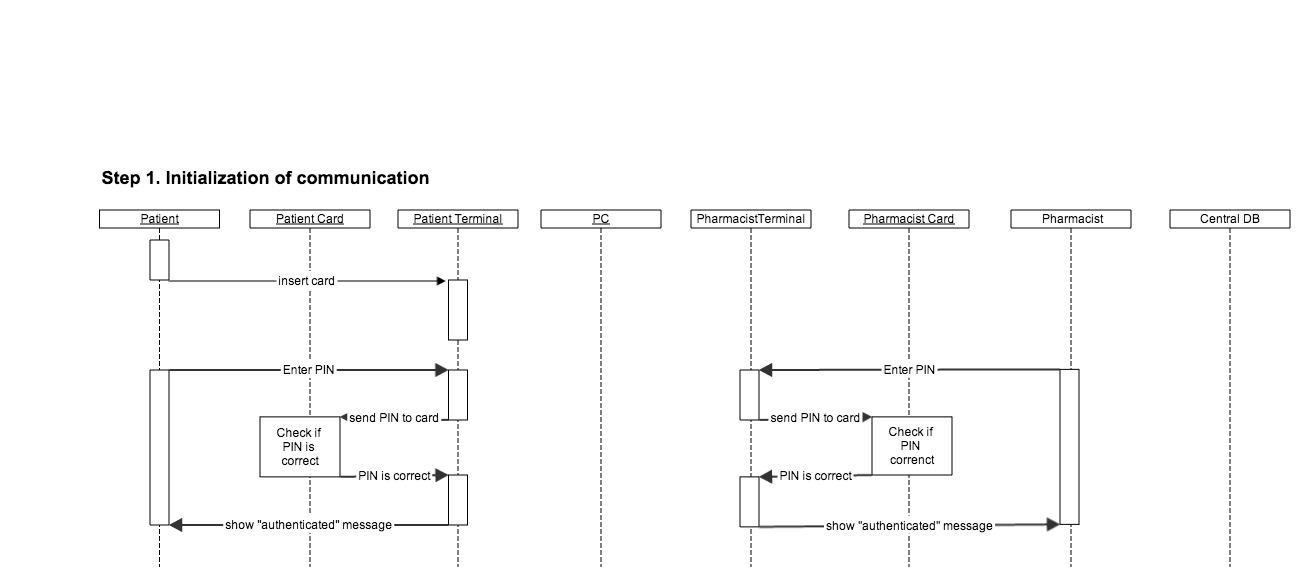
\includegraphics[scale=0.45]{s_d_1.png}
    \caption{Sequence diagram - step 1}
    \label{fig:s_q_step_1}
\end{figure} 

At the beginning, a patient puts his personal card to a terminal and he enters his PIN as usual, e.g. in the ATM. If the PIN is correct, the user can see appropriate message on the terminal screen. Also a pharmacist have to use his card and enters his PIN in the second terminal. Then, the system is ready to work. 

PINs are preventing from unauthorized usage of cards, e.g. when a card was stolen or lost.


\begin{figure}	
	\hspace*{-1.5in}
    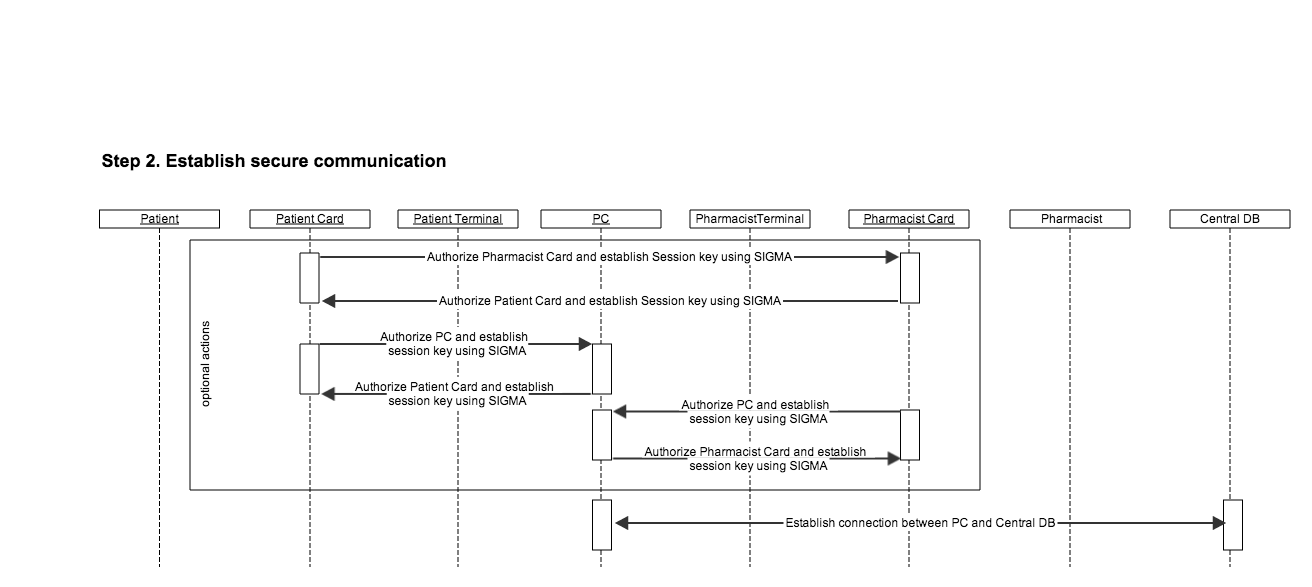
\includegraphics[scale=0.45]{s_d_2.png}
    \caption{Sequence diagram - step 2}
    \label{fig:s_q_step_2}
\end{figure} 

The second step, presented on the figure \ref{fig:s_q_step_2}, contains actions related with establishing secure communication  between the system parties. All the actions marked there, are optional and are not required for the system to work properly. Establishing a secure communication between the cards allows the participant to be sure, that the patient's and pharmacist's cards are not forged and they are authenticated to each other.
Similarly, suing the SIGMA protocol between a card (patient's or pharmacist's) and the application installed on the PC, allows to authorize the application by the card and the card by the application. These two sub-steps can be implemented, if a very-high level of the security is required. 

The communication between the application on the PC and the Central Database is performed in the way described in the Central Database Module Documentation.

\begin{figure}	
	\hspace*{-1.5in}
    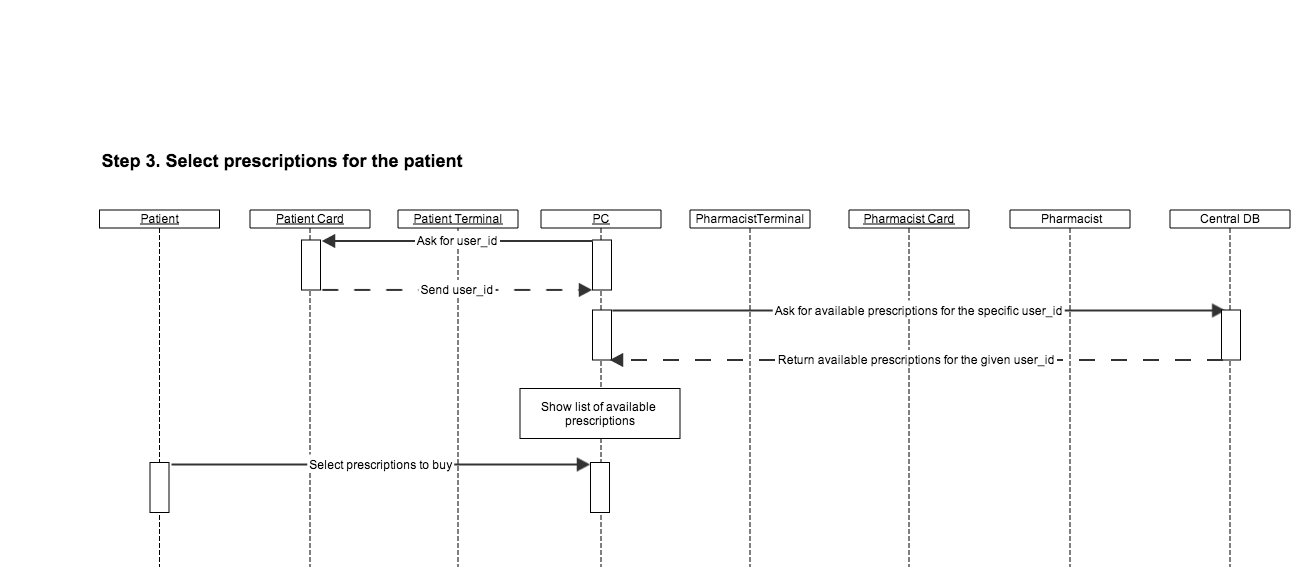
\includegraphics[scale=0.45]{s_d_3.png}
    \caption{Sequence diagram - step 3}
    \label{fig:s_q_step_3}
\end{figure} 

The figure \ref{fig:s_q_step_3} presents a point in the protocol, in which user's prescriptions are downloaded from the Central Database and are shown on the screen. After that the patient selects one or more of them to realize them.  User's identification data are stored on his card. They are used to authenticate the patient and to download appropriate prescriptions. 


\begin{figure}	
	\hspace*{-1.5in}
    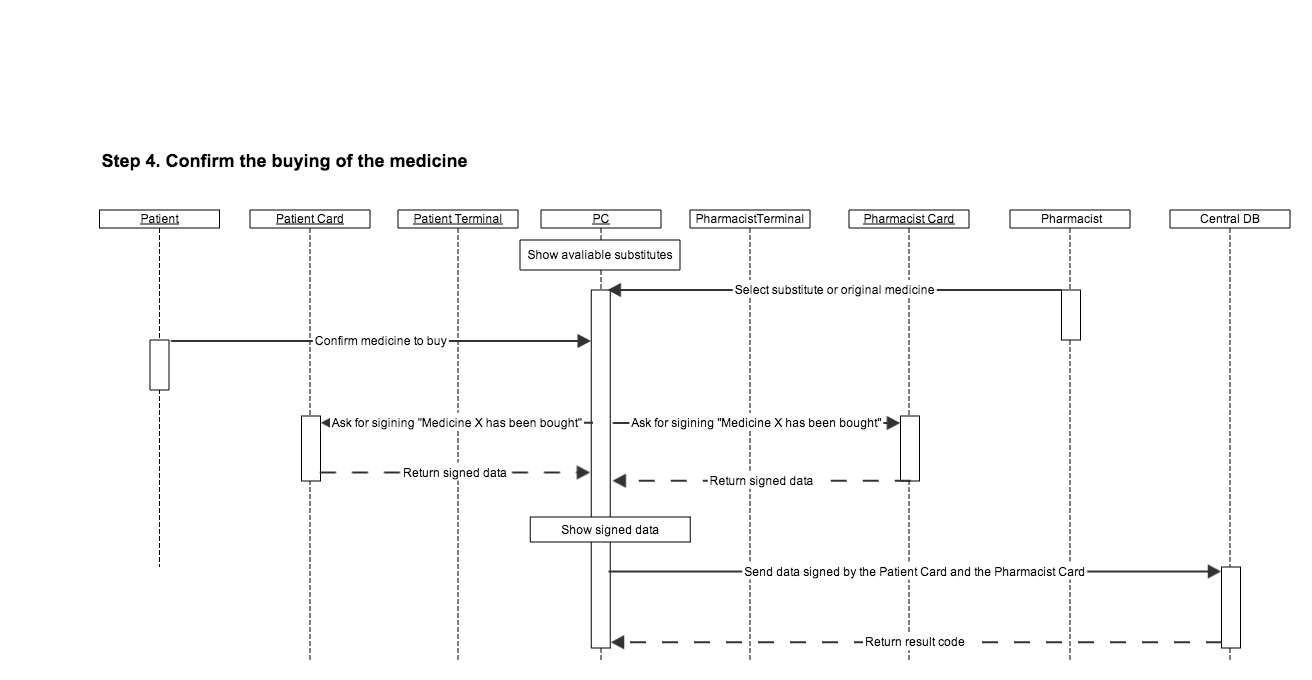
\includegraphics[scale=0.45]{s_d_4.png}
    \caption{Sequence diagram - step 4}
    \label{fig:s_q_step_4}
\end{figure} 

The last step is presented on the figure \ref{fig:s_q_step_4}. This scheme is repeated for the each prescription. At the beginning, the system shows available substitutions for the medicine. Then, the pharmacist can select original medicine or one of the substitutions and the patient can confirm this choose. 

Then, the application ask the patient and pharmacist cards to sign selected data. After it receives a response, it sends this signed data to the Central Database. The data are saved there. Because of that, it is  impossible to simulate buying process, without patient's personal card. The prescription's data have to be signed by the patient to be inserted into a database as a  bought prescription. Without a valid insert, the refoundation will not be granted. 

At the end of the protocol, all ephemeral keys are destroyed. 



